% \problemname{Minequake}
\problemname{Trzęsienia kopalni} % TODO: może lepszy tytuł?
\illustration{.4}{img/Goodluck_Mine.jpg}{%
  \emph{Goodluck Mine, Passage} by Ashley Dace. 
  License CC BY-SA 2.0.}

\noindent
% The fully autonomous microbreweries installed in the abandoned Dwarven mines of Moravia are truly a testament to the ingenuinity and craftsmanship of Dwarven engineering!
W pełni autonomiczne mikrobrowary zainstalowane w opuszczonych krasnoludzkich kopalniach na Morawach są prawdziwym świadectwem pomysłowości i kunsztu krasnoludzkiej inżynierii!
% Alas, sometimes earthquakes rattle the mines, leading to misaligned pipes and funnels spilling precious liquid on the floor.
Niestety, czasami trzęsienia ziemi wstrząsają kopalniami, co prowadzi do nieprawidłowego ustawienia rur i lejków, które rozlewają cenny płyn na podłogę.
% As the Exalted Warden of Brewery Safety it is your responsibility to turn off the machines in every hall in case of an earthquake.
Jako Najwyższy Strażnik Bezpieczeństwa Browaru masz obowiązek wyłączyć maszyny w każdej hali gdy nastąpi trzęsienie ziemi.

% Walking through tunnels takes time, 
Chodzenie po tunelach wymaga czasu, 
% so you will inevitably arrive late at many of the machines.
więc nieuchronnie spóźnisz się do wielu maszyn.
% This cannot be avoided, but you want to minimise the total amount of spilled liquid.
Nie da się tego uniknąć, ale chcesz zminimalizować całkowitą ilość rozlanego płynu.

\medskip
% The Dwarven mines consist of $n$~halls connected by $n-1$~tunnels.
Kopalnie Krasnoludów składają się z $n$~hal połączonych $n-1$~tunelami.
% The entire system is connected, so it is possible to get from any hall to any of the others.
Cały system jest spójny, więc możliwe jest dostanie się z każdej hali do każdej innej.
% It takes $1$~unit of time to traverse a tunnel.
Przemierzenie tunelu zajmuje $1$~jednostkę czasu.
% Switching off a machines and traversing a hall takes no time.
Wyłączenie maszyn i przemierzenie hali nie zajmuje żadnego czasu.
% In each hall, turning off the machines at time~$t$ after the earthquake spills $t$~liters of liquid.
W każdej hali wyłączenie maszyn w czasie~$t$ po trzęsieniu ziemi powoduje rozlanie $t$~litrów cieczy.
% There is exactly one earthquake, the earthquake affects all halls at the same time, and you may not switch off any machines before the earthquake.
Jest dokładnie jedno trzęsienie ziemi, które dotyka wszystkich hal jednocześnie i nie możesz wyłączyć żadnych maszyn ściśle przed trzęsieniem ziemi.
% You can start in any of the halls.
Możesz zacząć w dowolnej z hal.

\section*{Przykład}

% In sample input~$1$, the mines look like this:
W przykładowym wejściu~$1$, kopalnie wyglądają następująco:

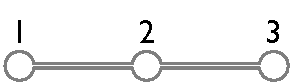
\includegraphics[width=.2\textwidth]{img/sample-1.pdf}

% If you start in hall~$2$ and visit the rest of the halls in the order $2$, $1$, $2$, $3$, then you can switch off their machines at time~$0$ (in hall $2$), time~$1$ (in hall $1$), and time~$3$ (in hall $3$).
Jeśli zaczynasz w hali~$2$ i odwiedzasz pozostałe hale w kolejności $2$, $1$, $2$, $3$, to możesz wyłączyć ich maszyny w czasie~$0$ (w hali $2$), czasie~$1$ (w hali $1$) oraz czasie~$3$ (w hali $3$).
% This wastes $0+1+3=4$~liters of liquid in total.
W ten sposób marnuje się łącznie $0+1+3=4$~litrów płynu.
% If instead you start in hall~$1$ and visit the halls in the order $1$, $2$, $3$, the total amount of liquid wasted is $0+1+2=3$~liters, which is better.
Jeśli zamiast tego zaczniesz w sali~$1$ i odwiedzisz sale w kolejności $1$, $2$, $3$, całkowita ilość zmarnowanego płynu wynosi $0+1+2=3$~litrów, co jest lepsze.

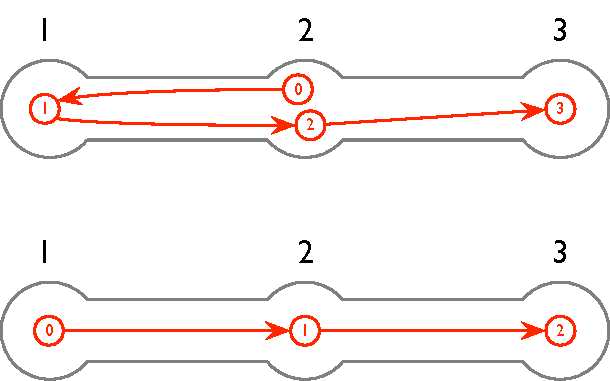
\includegraphics[width=.4\textwidth]{img/sample-1-ans.pdf}

\section*{Wejście}

% The first line of input consists of the integer $n$, denoting the number of halls.
W pierwszym wierszu wejścia znajduje się liczba całkowita $n$, oznaczająca liczbę hal.
% We assume that the halls are numbered $1$, $\ldots$, $n$.
Zakładamy, że hale są ponumerowane $1$, $\ldots$, $n$.
% The next $n-1$ lines each contain two space-separated integers $u$ and $v$ with 
W kolejnych $n-1$ wierszach znajdują się po dwie oddzielone spacjami liczby całkowite $u$ oraz $v$ spełniające
$1\leq u < v \leq n$, % constraint:hallnames
% meaning that there is a tunnel between hall~$u$ and hall~$v$.
oznaczające, że istnieje tunel między halą $u$ oraz halą $v$.

\section*{Wyjście}

% Print a single integer: the minimum amount of spilled liquid, in liters.
Wypisz jedną liczbę całkowitą: minimalną ilość rozlanego płynu, w litrach.

\section*{Ograniczenia i punktacja}

% We always have
Zawsze jest spełnione
$1\leq n\leq 10^5$. % constraint:n

% Your solution will be tested on a set of test groups, each worth a number of points.
Twoje rozwiązanie zostanie przetestowane na zestawie grup testowych, z których każda warta jest pewną liczbę punktów.
% Each test group contains a set of test cases.
Każda grupa testowa zawiera zestaw przypadków testowych.
% To get the points for a test group you need to solve all test cases in the test group.
Aby uzyskać punkty za grupę testową musisz rozwiązać wszystkie przypadki testowe w tej grupie.
% Your final score will be the maximum score of a single submission.
Twój ostateczny wynik będzie maksymalnym wynikiem pojedynczego zgłoszenia.

\medskip
\begin{tabular}{lll}
% Group & Points & Constraints \\\hline
Grupa & Punkty & Ograniczenia \\\hline
%   $1$ & $18$ & no hall has more than two tunnels\\
  $1$ & $18$ & żadna hala nie ma więcej niż dwa tunele\\
%   $2$ & $19$ & at most one hall has more than two tunnels\\
  $2$ & $19$ & co najwyżej jedna hala ma więcej niż dwa tunele\\
  $3$ & $20$ & $n\leq 10$\\
  $4$ & $21$ & $n\leq 1000$\\
%   $5$ & $22$ & \emph{No additional constraints}
  $5$ & $22$ & \emph{Brak dodatkowych ograniczeń}
\end{tabular}
